% Generated from the 4-node Stanford Dragon visualization run, job 337.
\begin{figure}[htbp]
  \centering
  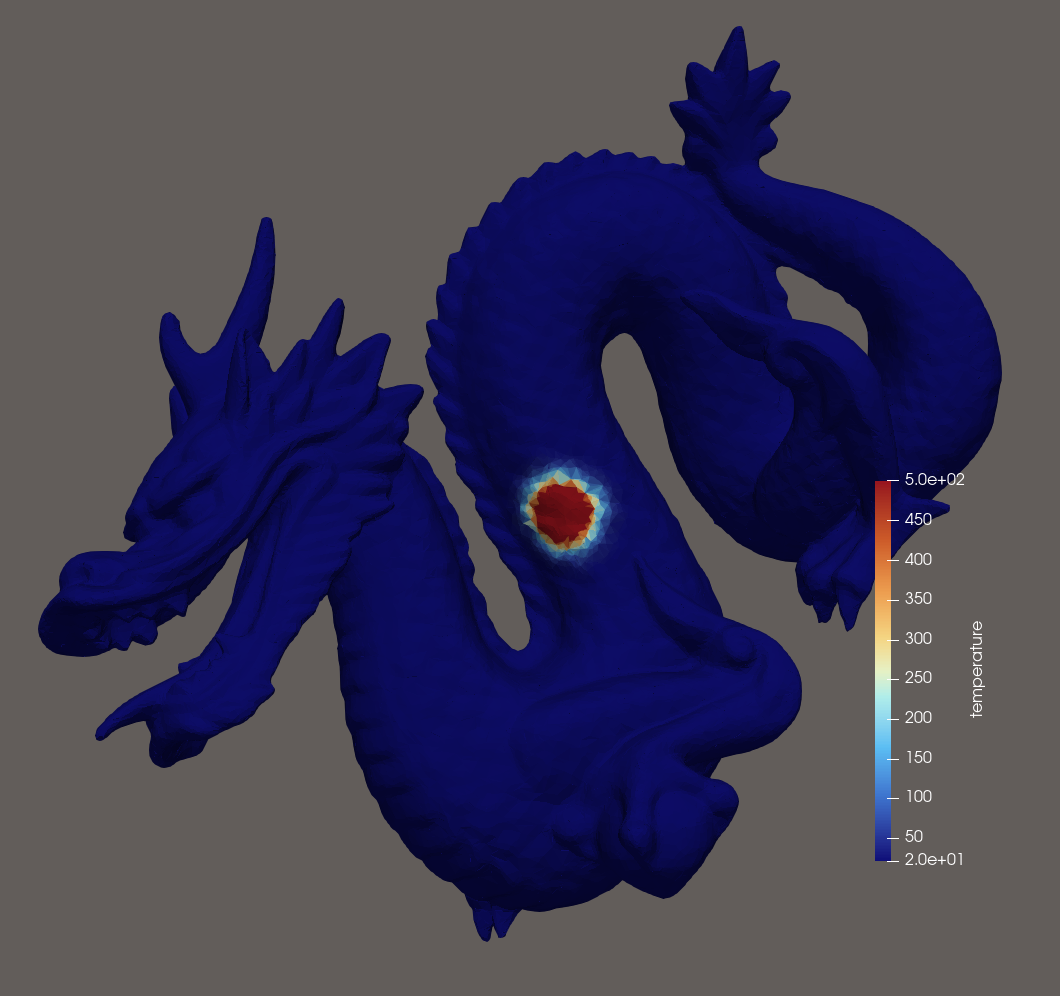
\includegraphics[width=0.88\linewidth]{figures/temperature_paraview.png}
  \caption{Розподіл температури на STL-поверхні Stanford Dragon після 12\,000 часових кроків, візуалізований у ParaView.
  Меш містить 115\,447 трикутних полігонів; температура кольором відповідає
  атрибуту полігона, а область джерела підтримується на рівні $500$.}
  \label{fig:temperature-n4}
\end{figure}

\begin{figure}[htbp]
  \centering
  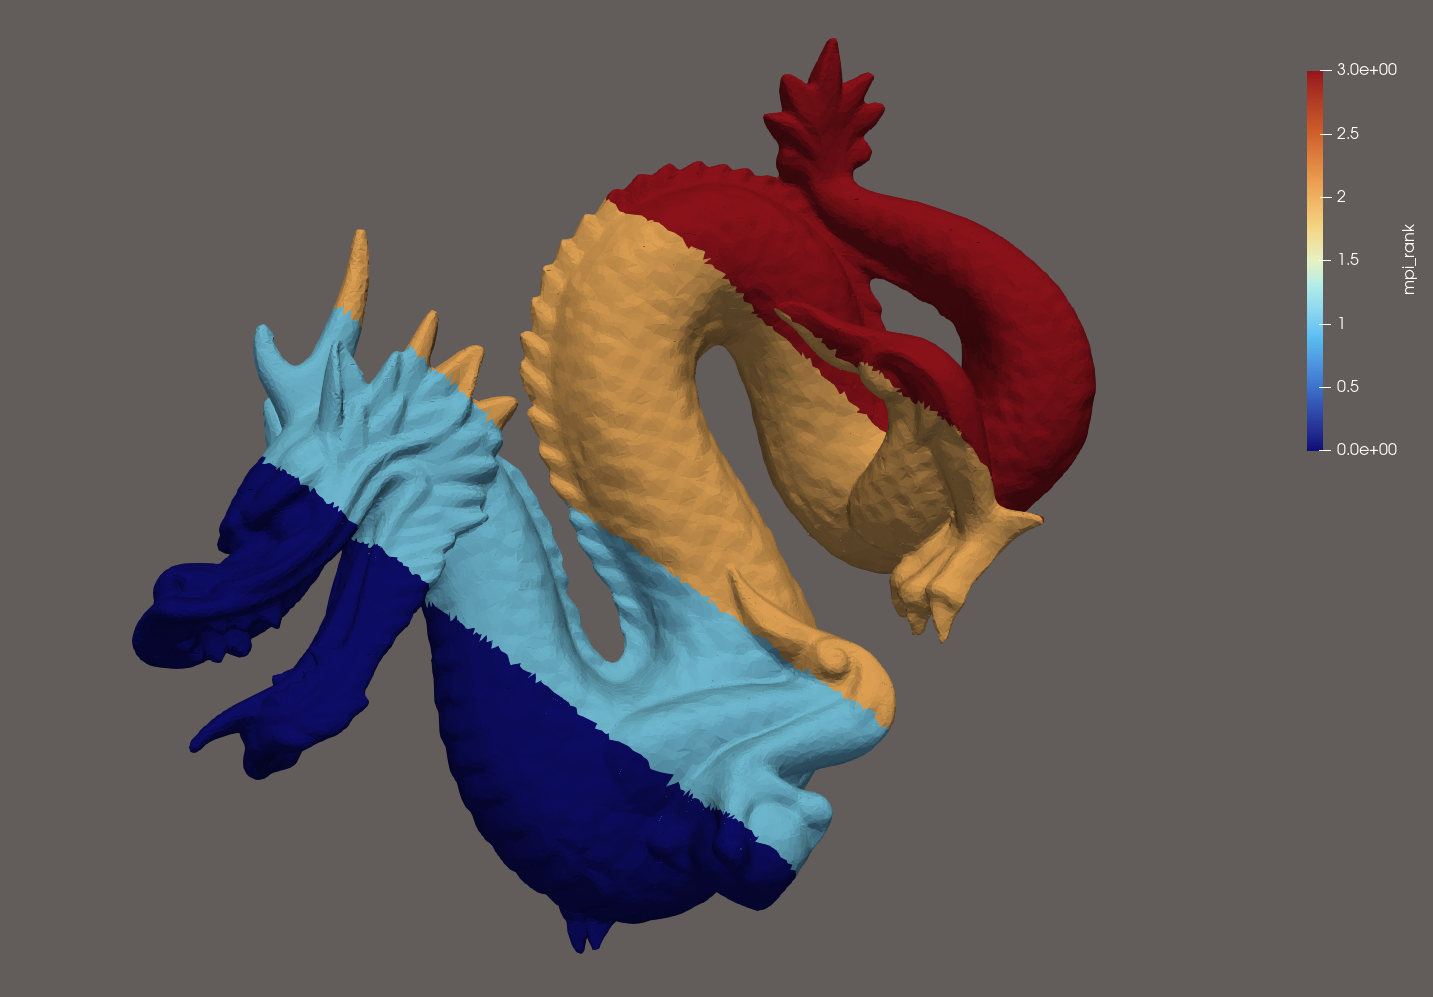
\includegraphics[width=0.48\linewidth]{figures/partition_paraview.png}
  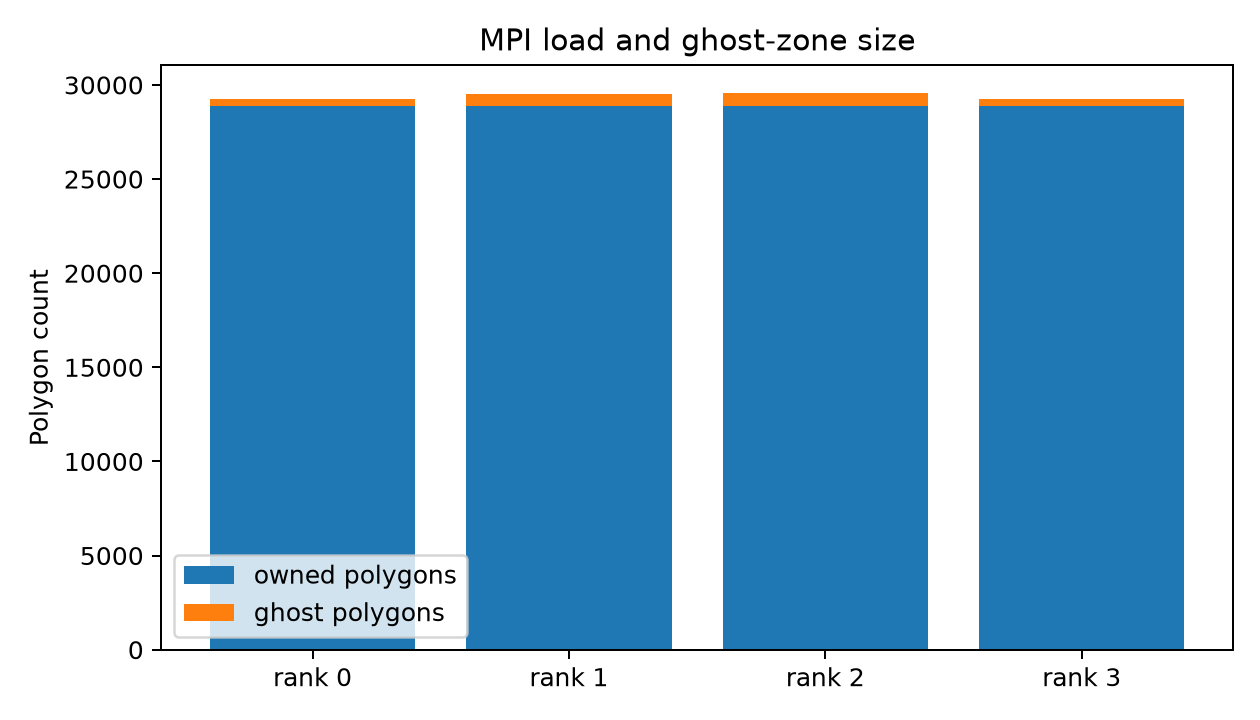
\includegraphics[width=0.48\linewidth]{figures/load_ghost_distribution.png}
  \caption{Просторове розбиття меша між чотирма MPI-процесами у ParaView та
  кількість власних і ghost-полігонів кожного процесу.}
  \label{fig:mpi-partition}
\end{figure}

\begin{figure}[htbp]
  \centering
  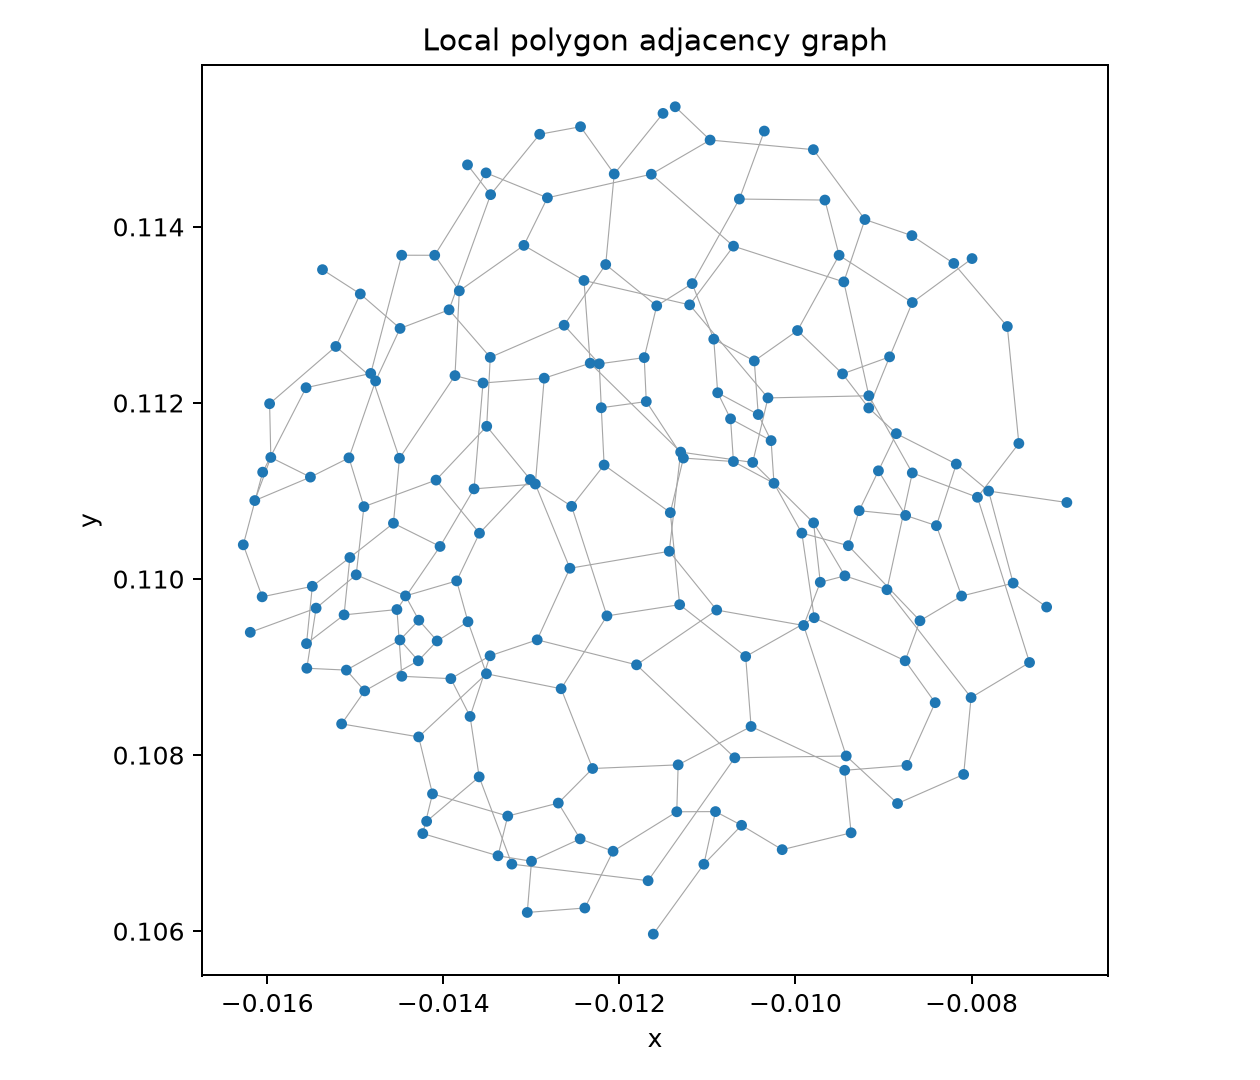
\includegraphics[width=0.62\linewidth]{figures/adjacency_graph.png}
  \caption{Локальний фрагмент графа сусідства трикутних полігонів.
  Лінія означає наявність спільного ребра, колір вершини --- MPI rank.}
  \label{fig:adjacency}
\end{figure}

\begin{figure}[htbp]
  \centering
  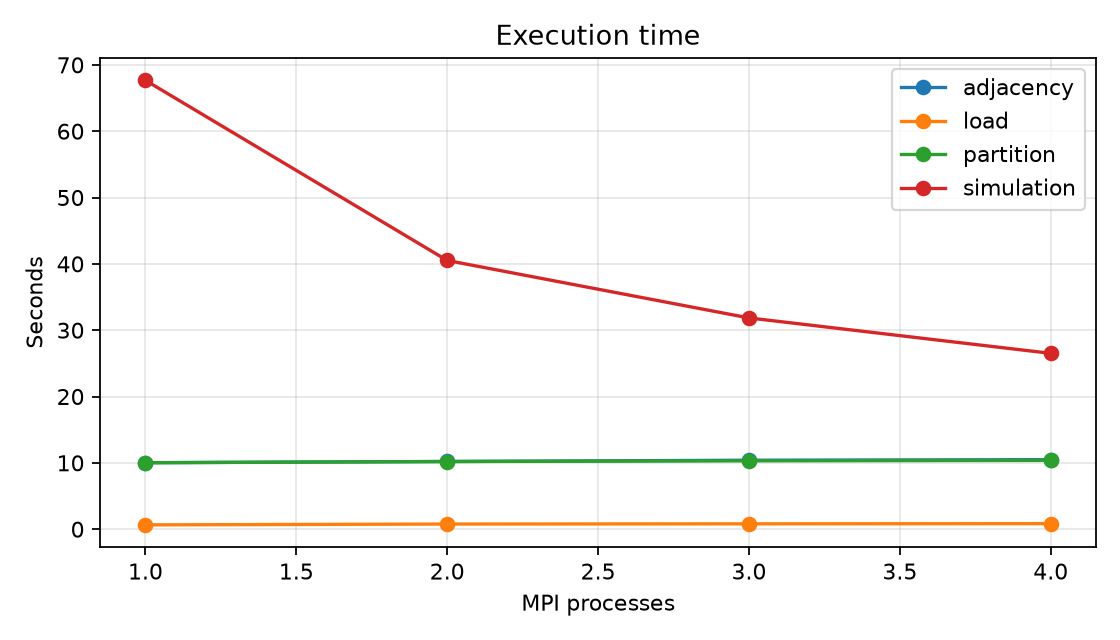
\includegraphics[width=0.48\linewidth]{figures/execution_time.png}
  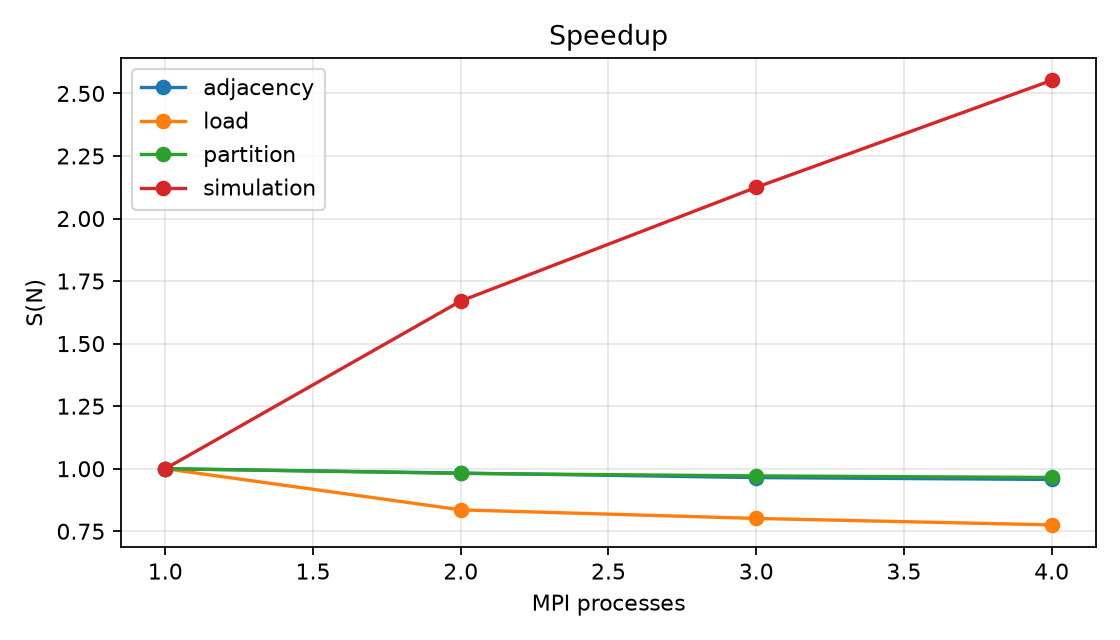
\includegraphics[width=0.48\linewidth]{figures/speedup.png}
  \caption{Медіанний час виконання та прискорення окремих режимів для Stanford Dragon,
  300 часових кроків і трьох повторів кожної конфігурації.}
  \label{fig:scaling}
\end{figure}
